% ----------------------------------------------------------
% Metodologia e Arquitetura do Sistema
% ----------------------------------------------------------
\chapter{Metodologia e Arquitetura do Sistema}

A plataforma emprega acionamento diferencial com o iRobot Roomba® 614 como base mecânica, controlada por Raspberry Pi 4 Model B (Ubuntu 22.04) sem microcontroladores intermediários, caracterizando \textit{Edge Computing}: sensoriamento, PID e atuação em malha única local \cite{siegwart2011introduction, macenski2022robot, zhang2022distributed}. O Roomba é acionado via cabo USB-Serial TTL (\textit{/dev/ttyUSB0}, 115200 bps), com alimentação do RPi4 isolada em bateria externa 5V para eliminar ruído elétrico dos motores (12V).

\section{Controle PID e Sensoriamento}

O erro de trajetória é extraído das 5 leituras binárias do módulo BFD-1000 por média ponderada com pesos $(-2,-1,0,1,2)$. O controlador opera a \textbf{20 Hz} ($\Delta t = 0{,}05$ s) segundo a formulação discreta \cite{ferreira2023differential, baluja2024design}:

\begin{equation}
    u(k) = K_p\, e(k) + K_i \sum_{i=0}^{k} e(i)\,\Delta t + K_d\, \frac{e(k) - e(k-1)}{\Delta t}
    \label{eq:pid_discreto}
\end{equation}

Os ganhos foram sintonizados empiricamente em campo (Tabela \ref{tab:pid_tuning}, Seção \ref{sec:resultados_pid}). Todo o código é implementado em Python (\texttt{rclpy}) em três pacotes ROS 2 \cite{amadi2024ros2control}: \textbf{\textit{roomba\_pi\_drivers}} (leitura GPIO → tópico \textit{/line\_sensor} a 20\,Hz; tradução de \textit{Twist} para protocolo serial); \textbf{\textit{roomba\_logic}} (nó PID \textit{pid\_controller\_node.py} e orquestrador de estados \textit{mission\_control\_pi.py} → tópico \textit{/cmd\_vel}); e \textbf{\textit{roomba\_bringup}} (\textit{launch files} com carga dinâmica dos ganhos).

\section{Arquitetura e Validação em Simulação}

As Figuras \ref{fig:diagrama_sistema} e \ref{fig:fluxograma} apresentam, respectivamente, a arquitetura de nós e o ciclo completo de execução da solução.

\begin{figure}[H]
\centering
\begin{minipage}[b]{0.47\textwidth}
    \centering
    \captionof{figure}{Diagrama de blocos da arquitetura do sistema.}
    \label{fig:diagrama_sistema}
    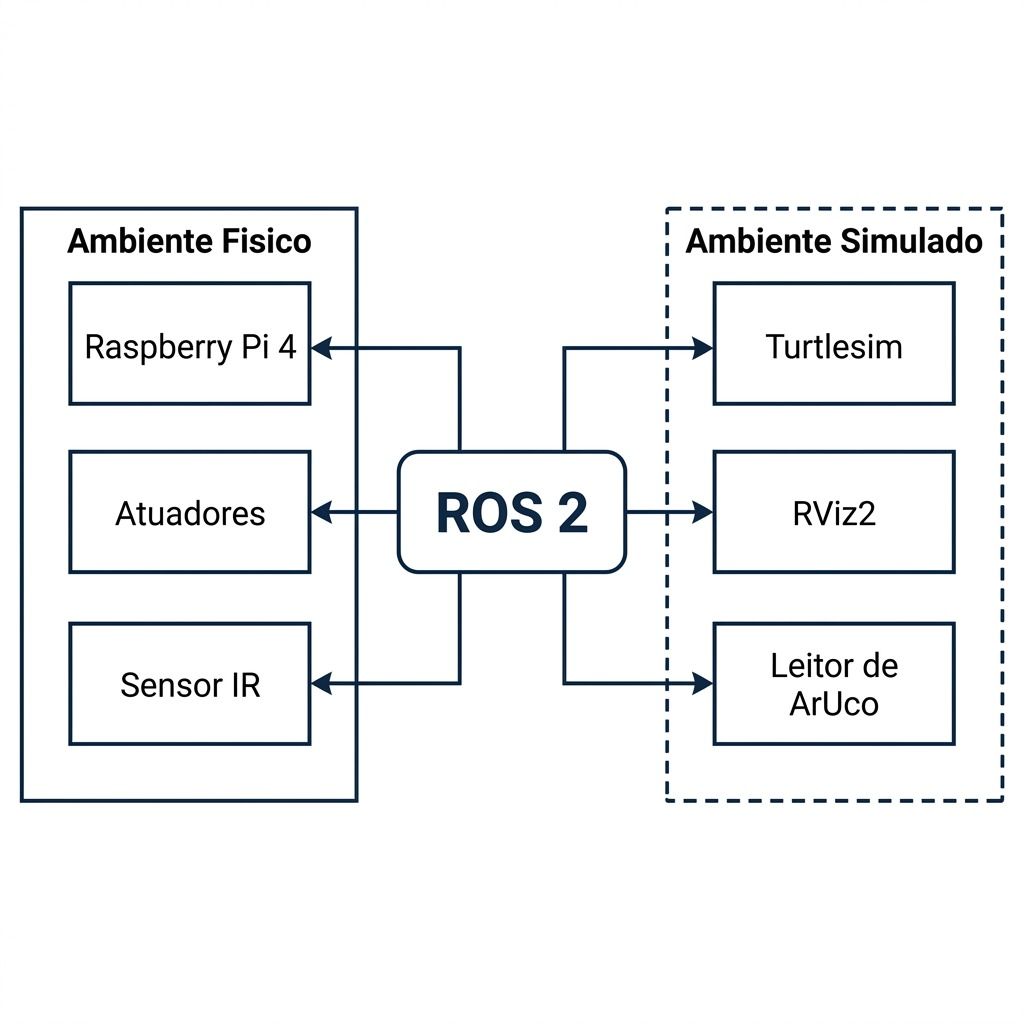
\includegraphics[width=\textwidth]{imagens/arquitetura_sistema}
    \legend{Fonte: Elaborado pelo autor.}
\end{minipage}
\hfill
\begin{minipage}[b]{0.50\textwidth}
    \centering
    \captionof{figure}{Fluxograma de funcionamento da solução.}
    \label{fig:fluxograma}
    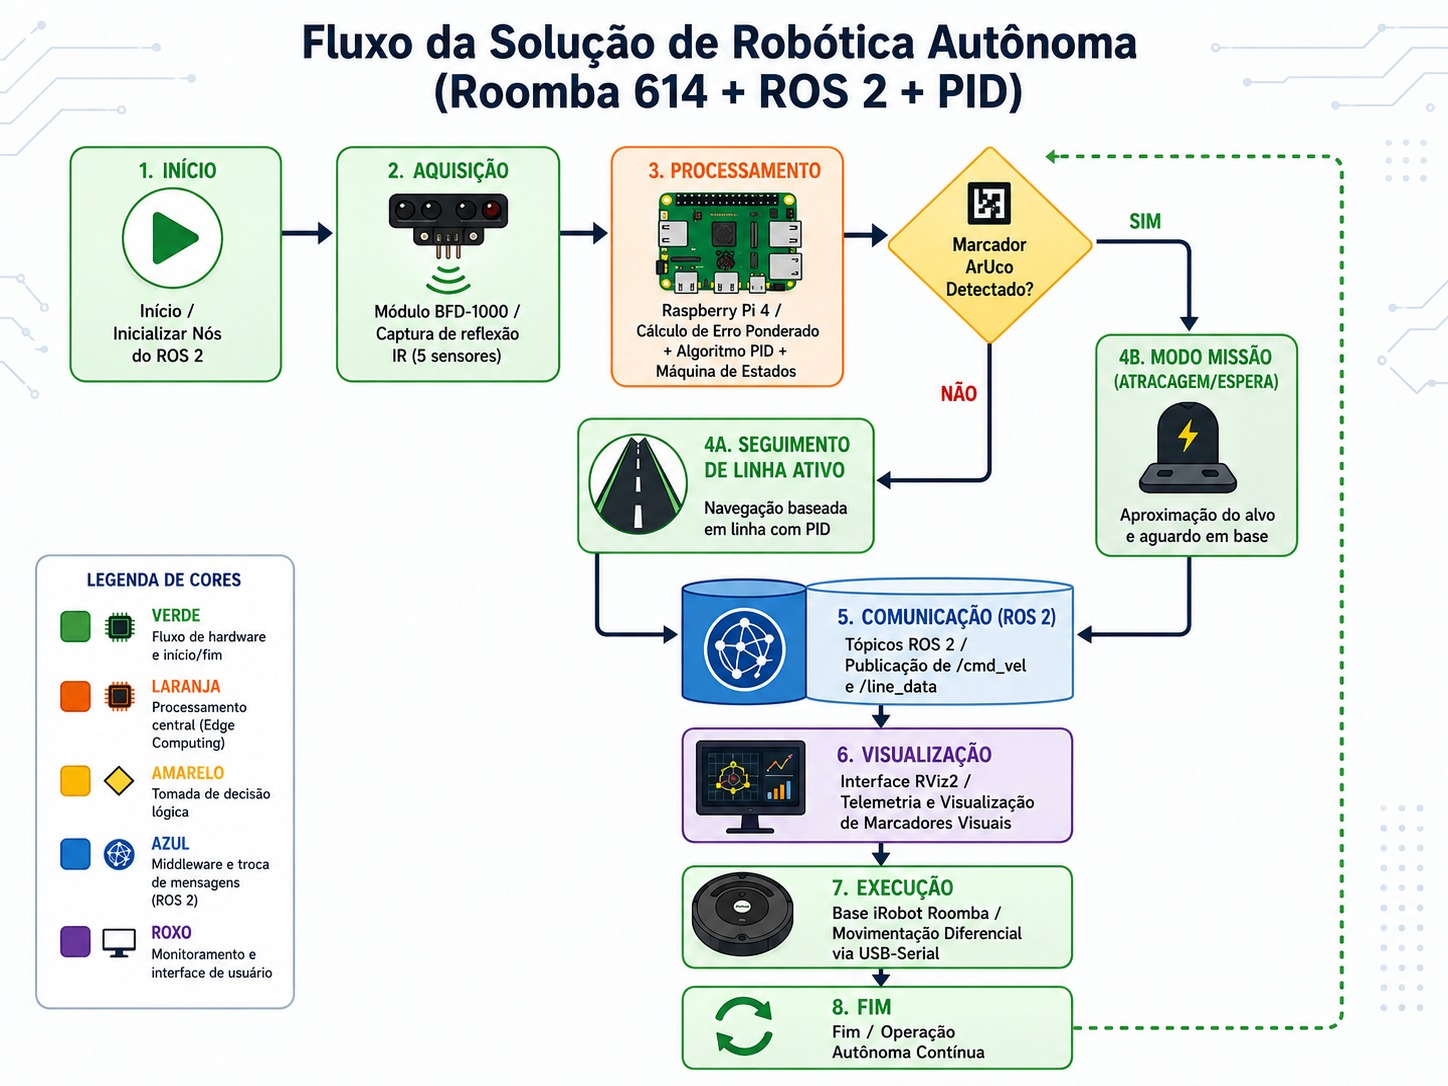
\includegraphics[width=\textwidth]{imagens/fluxograma_roomba_seguidor_linha}
    \legend{Fonte: Elaborado pelo autor.}
\end{minipage}
\end{figure}

Antes da implantação física, a lógica foi validada no \textit{Turtlesim} (2D, ROS 2 nativo), verificando roteamento de tópicos e equacionamento PID sem renderização 3D \cite{university2024labbook, stark2026development}; a ausência de modelagem de atrito e inércia exigiu \textit{fine-tuning} empírico posterior. Paralelamente, detecção de marcadores ArUco via OpenCV foi validada no \textit{RViz2} \cite{kalaitzakis2021fiducial, stangl2023analytical}, preparando a transição autônoma entre modos de navegação para integração física futura.
